\documentclass[a4paper,oneside]{article}

\usepackage[utf8]{inputenc}
\usepackage[T2A]{fontenc}
\usepackage[english,russian]{babel}

\usepackage{amsmath}
\usepackage{mathtools}
\usepackage{amsfonts}
\usepackage{enumitem}
\usepackage{amsthm}
\usepackage{minted}
\usepackage{underscore}
\setminted{fontsize=\small, breaklines=true, style=emacs, linenos}
\usepackage{graphicx}
\graphicspath{ {./images/} }
\usepackage{float}

\newtheorem{theorem}{Теорема}[subsection]
\newtheorem*{theorem*}{Теорема}

% --- Определение --- %
\theoremstyle{definition}
\newtheorem{definition}{Определение}[subsection]
\newtheorem*{definition*}{Определение}
% ------------------- %

\title{{Теория кодирования и сжатия информации}\\{Лабораторная работа №4}}
\author{Гущин Андрей, 431 группа, 1 подгруппа}
\date{\the\year{} г.}

\begin{document}

\maketitle

\section{Задача}

Разработать программу осуществляющую архивацию и разархивацию текстового
файла используя алгоритм адаптивного кода Хаффмана. Программы архивации и
разархивации должны быть представлены отдельно и работать независимо друг от
друга. Определить для данного шифра характеристики 1 (коэффициент сжатия) и 2
(скорость сжатия). К работе необходимо прикрепить отчет и программный проект.


\section{Алгоритм}

Алгоритм адаптивного кодирования Хаффмана заключается в обновлении дерева
кодирования для каждого нового введённого символа таким образом, чтобы
чаще встречающиеся символы в потоки получали наиболее эффективный код.

Основные свойства дерева, которые предстоит поддерживать при кодировании для
получения корректного кода --- это неявная нумерация и инвариантность. Неявная
нумерация --- все узлы пронумерованы по возрастанию по уровню, а также слева
направо. Инвариантность --- для любого веса $w$ все листья веса $w$ предшествуют
всем внутренним узлам веса $w$.

Алгоритм состоит из следующих шагов:
\begin{enumerate}
  \item
    Создать дерево из единственного узла NYT (Not Yet Transferred, Ещё не
    передано). Этот узел всегда будет иметь вес равный нулю. В выходной поток
    передадим один бит 0, который в данный момент будет означать начало
    кодирования;
  \item
    После получения нового символа из потока, закодируем передадим его в
    неизменном виде, после чего добавим в дерево, сохраняя свойства дерева;
  \item
    Если следующий символ ещё не встречался до этого, то в выходной поток
    передадим сначала код, соответствующий NYT, а затем сам символ в неизменном
    виде. Далее добавим этот символ в дерево, сохраняя свойства дерева;
  \item
    Если символ уже встречался, то увеличим его вес, а также веса всех его
    предков, сохраняя при этом свойства дерева.
\end{enumerate}

Перед увеличением веса любого из узлов, необходимо сначала поменять его местами
с лидером блока. Это действие не нужно производить только в том случае, если
лидером является прямой предок узла. Блок --- узлы одного веса. Лидер --- узел
блока с самым большим неявным номером.


\section{Тестирование}

Для проверки программы были использованы тестовые тексты 1 (рис.
\ref{fig:test_1}) и 6 (рис. \ref{fig:test_6}). Можно заметить,
что после распаковки архива полученный файл совпадает с исходным (проверка
с помощью утилиты diff). Также можно заметить, что для файлов малого размера
архив увеличивает их размер за счёт метаданных.

\begin{figure}[H]
  \centering
  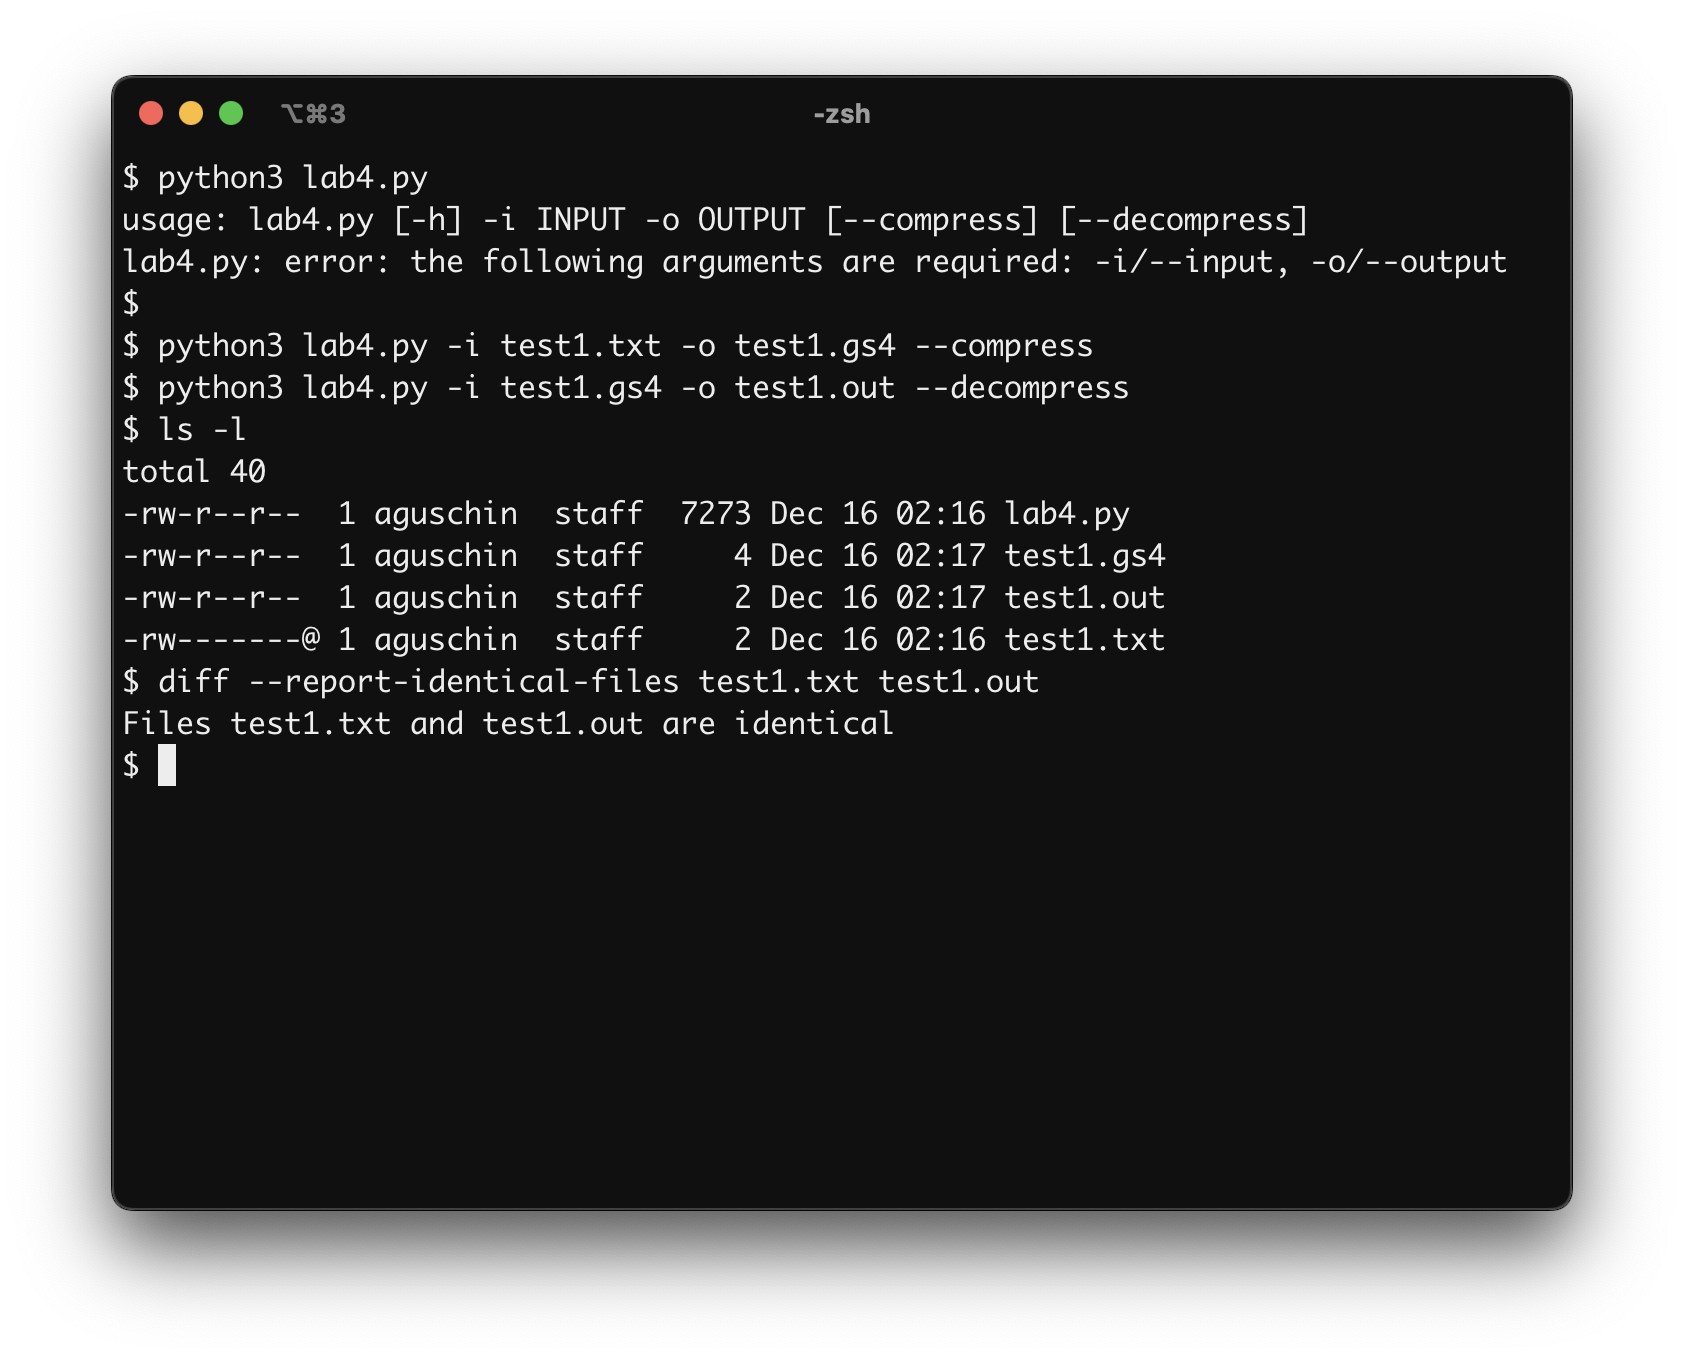
\includegraphics[width=0.9\textwidth]{test1.png}
  \caption{Сжатие текста Тест\_1.txt}
  \label{fig:test_1}
\end{figure}

\begin{figure}[H]
  \centering
  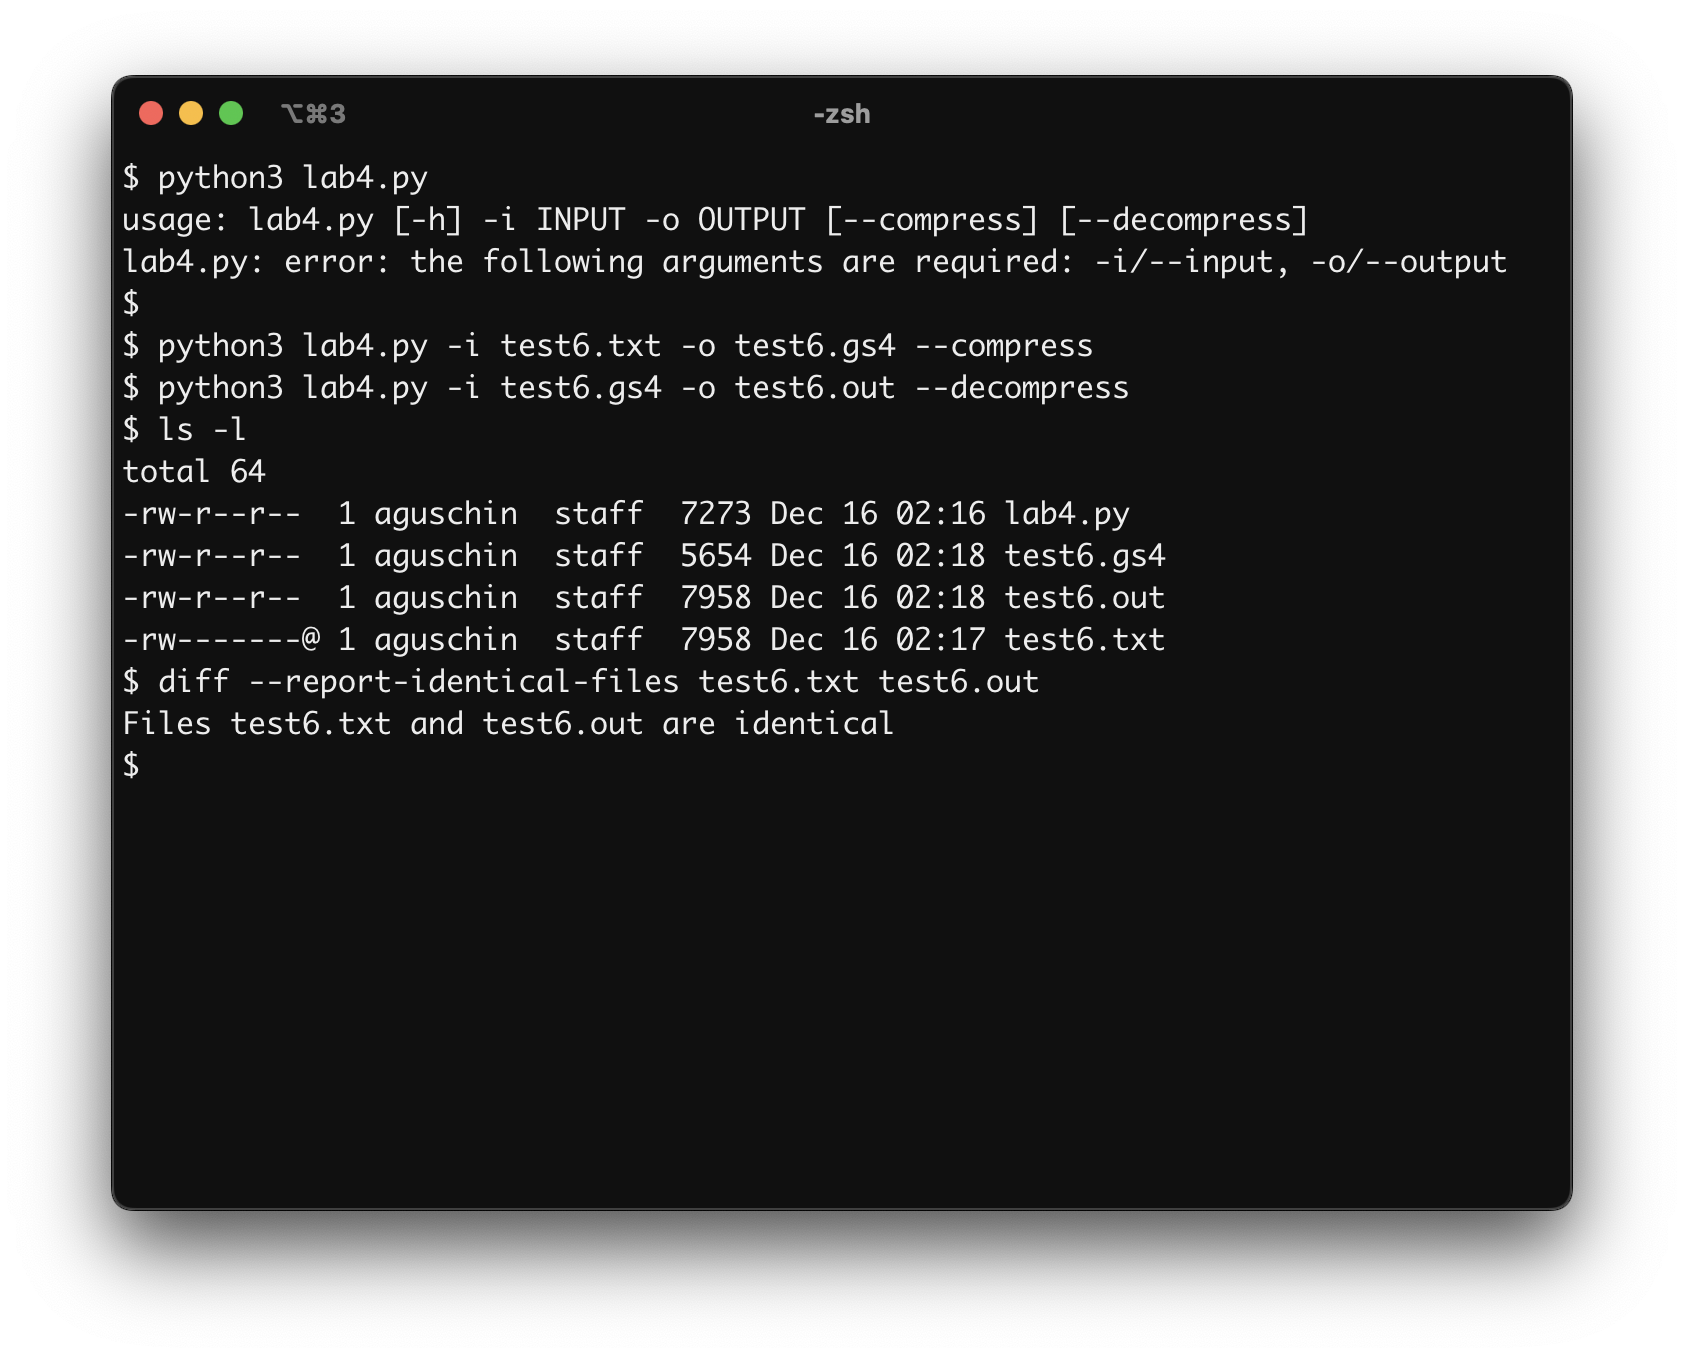
\includegraphics[width=0.9\textwidth]{test6.png}
  \caption{Сжатие текста Тест\_6.txt}
  \label{fig:test_6}
\end{figure}


\section{Вычисленные характеристики}

\subsection{Характеристика 1 (Коэффициент сжатия)}

Результаты применения программы к каждому из тестовых текстовых файлов занесены
в таблицу \ref{tbl:results}.

\begin{table}[H]
  \small
  \centering
  \begin{tabular}{|c|c|c|c|}
    \hline
    Название     & Исходный размер, байт & Сжатый размер, байт & Коэффициент \\ \hline \hline
    Тест\_1.txt  & 2           &      4      & 0.5     \\ \hline
    Тест\_2.txt  & 33          &     55      & 0.6     \\ \hline
    Тест\_3.txt  & 2739        &   1910      & 1.43403 \\ \hline
    Тест\_4.txt  & 330         &     65      & 5.07692 \\ \hline
    Тест\_5.txt  & 59          &    105      & 0.5619  \\ \hline
    Тест\_6.txt  & 7958        &   5654      & 1.4075  \\ \hline
    Тест\_7.txt  & 138245      &  85621      & 1.61462 \\ \hline
    Тест\_8.txt  & 574426      & 339607      & 1.69144 \\ \hline
    Тест\_9.txt  & 2752        &    346      & 7.95376 \\ \hline
    Тест\_10.txt & 2814        &    368      & 7.64674 \\ \hline
  \end{tabular}
  \caption{результаты тестирования}
  \label{tbl:results}
\end{table}

\subsection{Характеристика 2 (Скорость сжатия)}

Для тестирования скорости сжатия использовался тестовый файл Тест_7.txt
файл размера 138245 байт ($\approx$0.13 мегабайта). В результате пяти
последовательных запусков, среднее время запаковки файла составило 19.48
секунд, среднее время распаковки составило 9.46 секунд.

Таким образом, средняя скорость сжатия составила 0.00677 Мбайт в секунду, а
средняя скорость разжатия составила 0.01389 Мбайт в секунду.


\section{Реализация}

Программа реализована на языке программирования Python с использованием
стандартной библиотеки argparse для чтения параметров командной строки.

\subsection{Содержимое файла lab4.py}
\inputminted{python}{../../lab4-py/lab4.py}

\end{document}
